%%%%%%%%%%%%%%%%%%%%%%%%%%%%%%%%%%%%%%%%%%%%%%%%%%%%%%%%%%%%%%%%%%%%%
%
% CSCI 1430 Written Question Template
%
% This is a LaTeX document. LaTeX is a markup language for producing documents. 
% You will fill out this document, compile it into a PDF document, then upload the PDF to Gradescope. 
%
% To compile into a PDF on department machines:
% > pdflatex thisfile.tex
%
% If you do not have LaTeX, your options are:
% - Personal laptops (all common OS): http://www.latex-project.org/get/ 
% + VSCode extension: https://marketplace.visualstudio.com/items?itemName=James-Yu.latex-workshop
% - Online Tool: https://www.overleaf.com/ - most LaTeX packages are pre-installed here (e.g., \usepackage{}).
%
% If you need help with LaTeX, please come to office hours.
% Or, there is plenty of help online:
% https://en.wikibooks.org/wiki/LaTeX
%
% Good luck!
% The CSCI1430 staff
%
%%%%%%%%%%%%%%%%%%%%%%%%%%%%%%%%%%%%%%%%%%%%%%%%%%%%%%%%%%%%%%%%%%%%%

\documentclass[11pt]{article}

\usepackage[english]{babel}
\usepackage[utf8]{inputenc}
\usepackage{amssymb}
\usepackage{xcolor}
\usepackage[colorlinks = true,
            linkcolor = blue,
            urlcolor  = blue]{hyperref}
\usepackage[a4paper,margin=1.5in]{geometry}
\usepackage{stackengine,graphicx}
\usepackage{fancyhdr}
\setlength{\headheight}{15pt}
\usepackage{microtype}
\usepackage{times}
\usepackage[shortlabels]{enumitem}
\setlist[enumerate]{topsep=0pt}
\usepackage{amsmath}
\usepackage{framed}
\usepackage{mdframed}
\usepackage{xcolor}
\usepackage[most]{tcolorbox}

% a great python code format: https://github.com/olivierverdier/python-latex-highlighting
\usepackage{pythonhighlight}

\usepackage{trimclip,lipsum}

\frenchspacing
\setlength{\parindent}{0cm} % Default is 15pt.
\setlength{\parskip}{0.3cm plus1mm minus1mm}

\pagestyle{fancy}
\fancyhf{}
\lhead{Homework 1 Written Questions}
\rhead{CSCI 1430}
\lfoot{\textcolor{red}{\textbf{Only}
\ifcase\thepage
\or \textbf{instructions}
\or \textbf{generative AI use}
\or \textbf{A1 (a) (i) - (ii)}
\or \textbf{A1 (a) (iii) - (c)}
\or \textbf{A2 (a) - (b)}
\or \textbf{A2 (b)}
\or \textbf{A2 (c)}
\or \textbf{A3 (a) - (b)}
\or \textbf{A3 (c)}
\or \textbf{A3 (d)}
\or \textbf{A3 (e)}
\or \textbf{A4 (a) - (b)}
\or \textbf{A4 (c) - (d)}
\or \textbf{A5 (a) - (b)}
\or \textbf{A5 (c) - (e)}
\or \textbf{A5 (f) - (g)}
\or \textbf{feedback}
\else
\textbf{[ERROR: PAGE MISALIGNMENT]}
\fi
\textbf{should be on this page}
}}
\rfoot{\thepage~/ 16}


\date{}

\title{\vspace{-1cm}Homework 1 Written Questions}


\begin{document}
\maketitle
\thispagestyle{fancy}

\section*{Template Instructions}

This document is a template with specific answer regions and a fixed number of pages. Given large class sizes and limited TA time, the template helps the course staff to grade efficiently and still focus on the content of your submissions. Please help us in this task:
 
\begin{itemize}
  \item Make this document anonymous.
  
  \item Questions are in the orange boxes. Provide answers in the green boxes.
  \item Use the footer to check for correct page alignment.

  \item \textbf{Do NOT remove the answer box.}
  \item \textbf{Do NOT change the size of the answer box.}
  \item \textbf{Extra pages are not permitted unless otherwise specified.}
  \item \textbf{Template edits or page misalignment will lead to a 10 point deduction.}
\end{itemize}

\section*{Gradescope Submission}
\begin{itemize}
  \item Compile this document to a PDF and submit it to Gradescope.
  \item Pages will be automatically assigned to the right questions on Gradescope.
\end{itemize}

\section*{This Homework}
\begin{itemize}
    \item 5 questions \textbf{[12 + 8 + 13 + 14 + 7 = 54]}.
    \item Include code, images, and equations where appropriate.
\end{itemize}

% Please leave the pagebreak
\pagebreak

\section*{Declaration of Generative AI Use}

\subsection*{Reminder of Course Policy}

\begin{itemize}
    \item The use of GenAI tools (e.g., ChatGPT, Grammarly, Bard) for completing any part of this course is discouraged.
    \item Using these tools is not needed to be successful in the class and could be detrimental to your learning experience.
    \item If you use them, you must cite the tool you used and explain how you used it.
    \item If you do not cite the tool, it is an academic code violation.
    \item We will be using special tools to detect cases of unattributed GenAI use.
\end{itemize}

\subsection*{Student Declaration}

\subsubsection*{Have you used generative AI tools to complete this assignment:}

%%%%%%%%%%%%%% TODO %%%%%%%%%%%%%%%%%%%%

YES $\square$ NO $\blacksquare$ % change answer to \blacksquare

%%%%%%%%%%%%%%%%%%%%%%%%%%%%%%%%%%%%%%%%

\subsubsection*{If you answered YES above, describe what tools you used and what parts of the assignment you used them for below:}

%%%%%%%%%%%%%% TODO %%%%%%%%%%%%%%%%%%%%

\textit{Example: I used ChatGPT to debug my convolution implementation}

\pagebreak

\paragraph{Q1:} \textbf{[12 points]} 
We have been given special permission to use the telescope on the roof of Barus and Holley. Unfortunately, our fantastic image of the Orion nebula has noise caused by the imaging sensor: (\href{run:images/orion-noise.png}{orion-noise.png})

\begin{center}
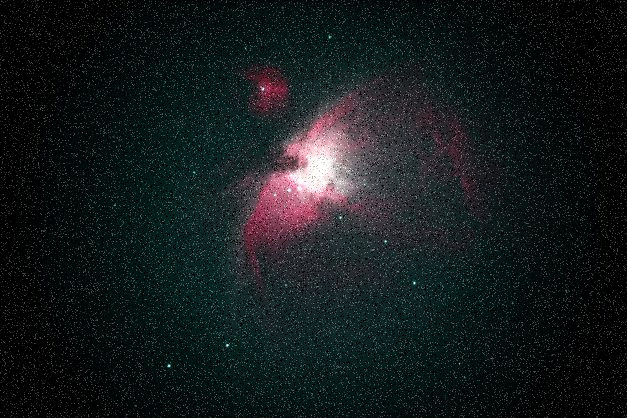
\includegraphics[width=0.5\textwidth,height=6cm,keepaspectratio]
{images/orion-noise.png}
\end{center}

One way to deal with this noise is with image convolution. 
Convolution is a type of image filtering that is a fundamental image processing tool.


\begin{enumerate}[(a)]
\item 
\begin{tcolorbox}[colback=orange!5!white,colframe=orange!75!black]
\emph{Explicitly describe} the input, transformation, and output components of 2D discrete convolution. Please be precise; define variables as need.
\end{tcolorbox}
\begin{enumerate}[(i)]
    \item \textbf{[2 points]} Input \textbf{[2--4 sentences]}
    \begin{tcolorbox}[colback=white!5!white,colframe=green!75!black]
        \setbox0=\hbox{\parbox[t]{\textwidth}{
        %%%%%%% ANSWER STARTS HERE %%%%%%%%%%%%%%%%%%%%%%%%%%%%
        
        
        %%%%%%% ANSWER ENDS HERE %%%%%%%%%%%%%%%%%%%%%%%%%%%%%%
        }}
        \clipbox{0pt \dimexpr\dp0-6\baselineskip\relax{} 0in 0pt}{\copy0}
\end{tcolorbox}
    
    \item \textbf{[2 points]} Transformation (how is the image transformed?) \textbf{[2--4 sentences]} 
\begin{tcolorbox}[colback=white!5!white,colframe=green!75!black]
    \setbox0=\hbox{\parbox[t]{\textwidth}{
        %%%%%%% ANSWER STARTS HERE %%%%%%%%%%%%%%%%%%%%%%%%%%%%
        
        
        %%%%%%% ANSWER ENDS HERE %%%%%%%%%%%%%%%%%%%%%%%%%%%%%%
        }}
        \clipbox{0pt \dimexpr\dp0-10\baselineskip\relax{} 0in 0pt}{\copy0}
\end{tcolorbox}
    
\pagebreak

    \item \textbf{[2 points]} Output \textbf{[2--4 sentences]}
    \begin{tcolorbox}[colback=white!5!white,colframe=green!75!black]
    \setbox0=\hbox{\parbox[t]{\textwidth}{
        %%%%%%% ANSWER STARTS HERE %%%%%%%%%%%%%%%%%%%%%%%%%%%%
        
        
        %%%%%%% ANSWER ENDS HERE %%%%%%%%%%%%%%%%%%%%%%%%%%%%%%
        }}
        \clipbox{0pt \dimexpr\dp0-8\baselineskip\relax{} 0in 0pt}{\copy0}
\end{tcolorbox}
    
\end{enumerate}


\item \textbf{[4 points]}
\begin{tcolorbox}[colback=orange!5!white,colframe=orange!75!black]
Describe two filter kernels that we may use with convolution, and give an example computer vision application that each enables. \textbf{[4--8 sentences]}
\end{tcolorbox}

\begin{tcolorbox}[colback=white!5!white,colframe=green!75!black]
\setbox0=\hbox{\parbox[t]{\textwidth}{
        %%%%%%% ANSWER STARTS HERE %%%%%%%%%%%%%%%%%%%%%%%%%%%%


        %%%%%%% ANSWER ENDS HERE %%%%%%%%%%%%%%%%%%%%%%%%%%%%%%
}}
\clipbox{0pt \dimexpr\dp0-13\baselineskip\relax{} 0in 0pt}{\copy0}
\end{tcolorbox}

\item \textbf{[2 point]}
\begin{tcolorbox}[colback=orange!5!white,colframe=orange!75!black]
What kind of filter might we use to de-noise our image of the Orion nebula, and why? \textbf{[2--3 sentences]}
\end{tcolorbox}
\begin{tcolorbox}[colback=white!5!white,colframe=green!75!black]
    \setbox0=\hbox{\parbox[t]{\textwidth}{
    %%%%%%% ANSWER STARTS HERE %%%%%%%%%%%%%%%%%%%%%%%%%%%%
        
        
    %%%%%%% ANSWER ENDS HERE %%%%%%%%%%%%%%%%%%%%%%%%%%%%%%
    }}
    \clipbox{0pt \dimexpr\dp0-6\baselineskip\relax{} 0in 0pt}{\copy0}
\end{tcolorbox}

\pagebreak


\end{enumerate}

% %%%%%%%%%%%%%%%%%%%%%%%%%%%%%%%%%%%

% Please leave the pagebreak
\pagebreak
\paragraph{Q2:} \textbf{[8 points]} Now that we've de-noised our image of the Orion nebula, let's explore filtering techniques more closely. Two kinds of linear filtering are correlation and convolution.

\begin{enumerate}[(a)]

    \item \textbf{[3 points]} 
    \begin{tcolorbox}[colback=orange!5!white,colframe=orange!75!black]
    What is different between convolution and correlation? Include differences in their algebraic properties. When might we use each? \textbf{[5--6 sentences]}
    \end{tcolorbox}
    
    \begin{tcolorbox}[colback=white!5!white,colframe=green!75!black]
    \setbox0=\hbox{\parbox[t]{\textwidth}{
        %%%%%%% ANSWER STARTS HERE %%%%%%%%%%%%%%%%%%%%%%%%%%%%

        
        %%%%%%% ANSWER ENDS HERE %%%%%%%%%%%%%%%%%%%%%%%%%%%%%%
    }}
    \clipbox{0pt \dimexpr\dp0-14\baselineskip\relax{} 0in 0pt}{\copy0}
    \end{tcolorbox}
    
    \item \textbf{[4 points]}
    To solidify our understanding of the distinction between correlation and convolution, we will process another image.
    
    \begin{tcolorbox}[colback=orange!5!white,colframe=orange!75!black]
    Devise a scenario in which the output of correlation and convolution differ.
    
    Write code that loads an image and produces two distinct images, one from convolution and one from correlation on some kernel of your choice. Then, compute the difference of the two images and display it as well.
    
    Specify your kernel, and provide the input image and two output results. Then, use your understanding of convolution and correlation to explain the outputs. \textbf{[2--4 sentences]}
    \end{tcolorbox}
    
    \emph{Consider \href{https://docs.scipy.org/doc/scipy/reference/generated/scipy.signal.convolve2d.html}{$scipy.signal.convolve2d$} and \href{https://docs.scipy.org/doc/scipy/reference/generated/scipy.signal.correlate2d.html}{$scipy.signal.correlate2d$} to experiment!}
    

\begin{tcolorbox}[colback=white!5!white,colframe=green!75!black,breakable]
    
\includegraphics[width=0.5\textwidth,height=7cm,keepaspectratio]{images/TODO_orig_img.png}
    
\includegraphics[width=0.5\textwidth,height=7cm,keepaspectratio]{images/TODO_difference.png}\\
    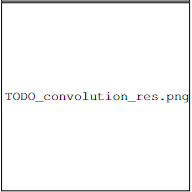
\includegraphics[width=0.5\textwidth,height=7cm,keepaspectratio]{images/TODO_convolution_res.png}
    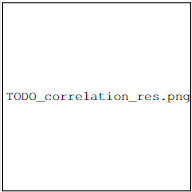
\includegraphics[width=0.5\textwidth,height=7cm,keepaspectratio]{images/TODO_correlation_res.png}
    
    \setbox0=\hbox{\parbox[t]{\textwidth}{
    %%%%%%% ANSWER STARTS HERE %%%%%%%%%%%%%%%%%%%%%%%%%%%%

    TODO: Your answer for (b) here %%%%%% Remove this line in your answer! %%%%%%
    
    %%%%%%% ANSWER ENDS HERE %%%%%%%%%%%%%%%%%%%%%%%%%%%%%%
    }}
    \clipbox{0pt \dimexpr\dp0-12\baselineskip\relax{} 0in 0pt}{\copy0}
\end{tcolorbox}

\pagebreak

    \item \textbf{[1 point]} 
    \begin{tcolorbox}[colback=orange!5!white,colframe=orange!75!black]
    Consider a situation where we are applying two different filters sequentially to an image.
    
    How will the output image change depending on the order in which we apply the filters? Will the behavior be different for convolution versus correlation? \textbf{[1--2 sentences]}
    \end{tcolorbox}

    \begin{tcolorbox}[colback=white!5!white,colframe=green!75!black]
    \setbox0=\hbox{\parbox[t]{\textwidth}{
        %%%%%%% ANSWER STARTS HERE %%%%%%%%%%%%%%%%%%%%%%%%%%%%

        
        %%%%%%% ANSWER ENDS HERE %%%%%%%%%%%%%%%%%%%%%%%%%%%%%%
    }}
    \clipbox{0pt \dimexpr\dp0-14\baselineskip\relax{} 0in 0pt}{\copy0}
    \end{tcolorbox}

\end{enumerate}

% %%%%%%%%%%%%%%%%%%%%%%%%%%%%%%%%%%%

% Please leave the page break
\pagebreak

\paragraph{Q3:} \textbf{[13 points]} While exploring Brown CS's history in the halls of CIT, we happen upon Nancy: a DEC VAX 11/780. So struck by its beauty, we decide to take an artful photo with our camera. Modern digital sensors have many megapixels, so we resize it to make the file smaller.

\begin{tabular}{c c}
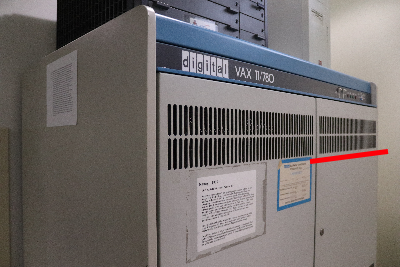
\includegraphics[width=0.49\textwidth,height=7cm,keepaspectratio]{images/poor_nancy_markup.png} &
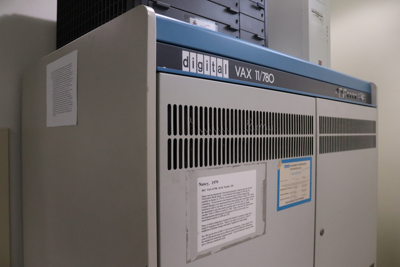
\includegraphics[width=0.49\textwidth,height=7cm,keepaspectratio]{images/poor_nancy_better.png} \\
Resized image & Depiction of original (\emph{not original file})
\end{tabular}

%%%%%%%%%%%%%%%%%%%%%%%%%%%%%%%%%%%

\begin{enumerate}[(a)]
\item \textbf{[3 points]} Oh no! What happened to Nancy? There are weird artifacts in the vents (above red line)---these definitely weren't there in the original photo. Plus, if we look closely, the white label text is less smooth and there are jagged lines.
    
    \begin{tcolorbox}[colback=orange!5!white,colframe=orange!75!black]
    What is this phenomenon called, and why did it happen? \textbf{[2--4 sentences]}
    \end{tcolorbox}
    \begin{tcolorbox}[colback=white!5!white,colframe=green!75!black]
    \setbox0=\hbox{\parbox[t]{\textwidth}{
    %%%%%%% ANSWER STARTS HERE %%%%%%%%%%%%%%%%%%%%%%%%%%%%

    TODO: Your answer for (a) here %%%%%% Remove this line in your answer! %%%%%%

    %%%%%%% ANSWER ENDS HERE %%%%%%%%%%%%%%%%%%%%%%%%%%%%%%
    }}
    \clipbox{0pt \dimexpr\dp0-7\baselineskip\relax{} 0in 0pt}{\copy0}
    \end{tcolorbox}

    \item \textbf{[3 points]}
    \begin{tcolorbox}[colback=orange!5!white,colframe=orange!75!black]
    How might we fix this issue with filtering? Describe the process, and explain why it works. \textbf{[2--4 sentences]}
    \end{tcolorbox}
    \begin{tcolorbox}[colback=white!5!white,colframe=green!75!black]
    \setbox0=\hbox{\parbox[t]{\textwidth}{
    %%%%%%% ANSWER STARTS HERE %%%%%%%%%%%%%%%%%%%%%%%%%%%%

    TODO: Your answer for (b) here %%%%%% Remove this line in your answer! %%%%%%

    %%%%%%% ANSWER ENDS HERE %%%%%%%%%%%%%%%%%%%%%%%%%%%%%%
    }}
    \clipbox{0pt \dimexpr\dp0-7\baselineskip\relax{} 0in 0pt}{\copy0}
    \end{tcolorbox}

\item \textbf{[3 points]}
\begin{tcolorbox}[colback=orange!5!white,colframe=orange!75!black]
Which of the following kernels is high pass, low pass, or neither?
\end{tcolorbox}

\emph{Note:} To fill in boxes, replace `\textbackslash square' with `\textbackslash blacksquare' for your answer.

\begin{enumerate}[(i)]
\item
 $\begin{bmatrix}
    1 & 0 & -1 \\
    1 & 0 & -1 \\
    1 & 0 & -1 \\
 \end{bmatrix}$
\begin{tcolorbox}[colback=white!5!white,colframe=green!75!black]
%%%%%%% ANSWER STARTS HERE %%%%%%%%%%%%%%%%%%%%%%%%%%%%
TODO: Select the appropriate answer. %%%%%% Remove this line in your answer! %%%%%%

\begin{tabular}[h]{ll}
$\square$ & High pass \\
$\square$ & Low pass \\
$\square$ & Neither \\
\end{tabular}

%%%%%%% ANSWER ENDS HERE %%%%%%%%%%%%%%%%%%%%%%%%%%%%%%
\end{tcolorbox}

\item
 $\begin{bmatrix}
    \frac{1}{9} & \frac{1}{9} & \frac{1}{9} \\
    \frac{1}{9} & \frac{1}{9} & \frac{1}{9} \\
    \frac{1}{9} & \frac{1}{9} & \frac{1}{9}
 \end{bmatrix}$
 \begin{tcolorbox}[colback=white!5!white,colframe=green!75!black]

%%%%%%% ANSWER STARTS HERE %%%%%%%%%%%%%%%%%%%%%%%%%%%%
TODO: Select the appropriate answer. %%%%%% Remove this line in your answer! %%%%%%

\begin{tabular}[h]{ll}
$\square$ & High pass \\
$\square$ & Low pass \\
$\square$ & Neither \\
\end{tabular}

%%%%%%% ANSWER ENDS HERE %%%%%%%%%%%%%%%%%%%%%%%%%%%%%%
%%%%%%% ANSWER STARTS HERE %%%%%%%%%%%%%%%%%%%%%%%%%%%%
%%%%%%% ANSWER ENDS HERE %%%%%%%%%%%%%%%%%%%%%%%%%%%%%%
\end{tcolorbox}

\item
$\begin{bmatrix}
    -\frac{1}{9} & -\frac{1}{9} & -\frac{1}{9} \\
    -\frac{1}{9} & \frac{8}{9} & -\frac{1}{9} \\
    -\frac{1}{9} & -\frac{1}{9} & -\frac{1}{9}
  \end{bmatrix}$
  \begin{tcolorbox}[colback=white!5!white,colframe=green!75!black]
  
TODO: Select the appropriate answer. %%%%%% Remove this line in your answer! %%%%%%

\begin{tabular}[h]{ll}
$\square$ & High pass \\
$\square$ & Low pass \\
$\square$ & Neither \\
\end{tabular}
\end{tcolorbox}
\end{enumerate}

\pagebreak

\item \textbf{[2 points]}
We decide to test if we can recognize which kind of filter has been used to achieve a target output image.

\begin{tcolorbox}[colback=orange!5!white,colframe=orange!75!black]
Given the input image below, identify the kind of filter.
\end{tcolorbox}

\raisebox{\baselineskip-\height}{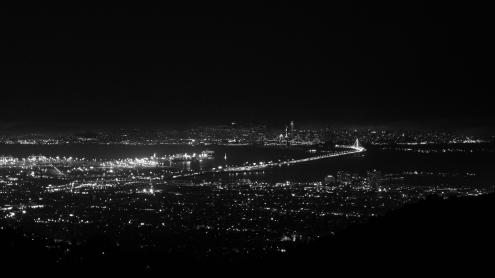
\includegraphics[width=0.5\textwidth,height=7cm,keepaspectratio]{images/q3img0.png}}

\begin{enumerate}[(i)]
\item
Output image 1:\\
\raisebox{\baselineskip-\height}{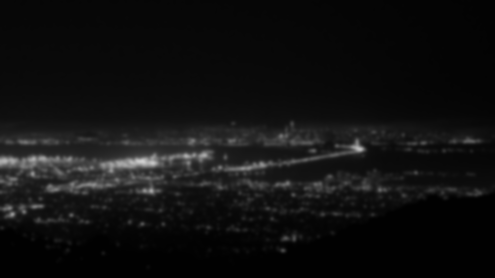
\includegraphics[width=0.5\textwidth,height=7cm,keepaspectratio]{images/q3img1.png}}
\begin{tcolorbox}[colback=white!5!white,colframe=green!75!black]
%%%%%%% ANSWER STARTS HERE %%%%%%%%%%%%%%%%%%%%%%%%%%%%
TODO: Select the appropriate answer. %%%%%% Remove this line in your answer! %%%%%%

\begin{tabular}[h]{lc}
$\square$ & High pass \\
$\square$ & Low pass \\
\end{tabular}
%%%%%%% ANSWER ENDS HERE %%%%%%%%%%%%%%%%%%%%%%%%%%%%%%
\end{tcolorbox}

\item
Output image 2 (adjusted for easier visualization):\\
\raisebox{\baselineskip-\height}{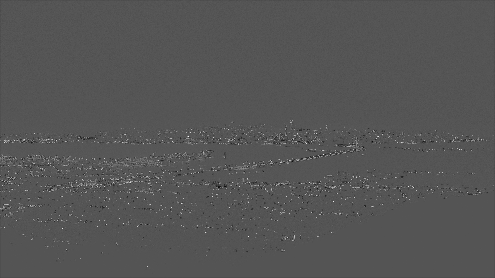
\includegraphics[width=0.5\textwidth,height=7cm,keepaspectratio]{images/q3img2.png}}
\begin{tcolorbox}[colback=white!5!white,colframe=green!75!black]
%%%%%%% ANSWER STARTS HERE %%%%%%%%%%%%%%%%%%%%%%%%%%%%
TODO: Select the appropriate answer. %%%%%% Remove this line in your answer! %%%%%%

\begin{tabular}[h]{lc}
$\square$ & High pass \\
$\square$ & Low pass \\
\end{tabular}
%%%%%%% ANSWER ENDS HERE %%%%%%%%%%%%%%%%%%%%%%%%%%%%%%
\end{tcolorbox}
\end{enumerate}

\pagebreak
\item \textbf{[2 points]}
\begin{tcolorbox}[colback=orange!5!white,colframe=orange!75!black]
Which of the following statements are true? (Check all that apply).
\end{tcolorbox}

\begin{tcolorbox}[colback=white!5!white,colframe=green!75!black]
%%%%%%% ANSWER STARTS HERE %%%%%%%%%%%%%%%%%%%%%%%%%%%%
TODO: Select all that apply. %%%%%% Remove this line in your answer! %%%%%%

\begin{tabular}[h]{ll}
$\square$ & High pass filter kernels will always contain at least one negative \\
& number \\
$\square$ & A Gaussian filter is an example of a low pass filter \\
$\square$ & A high pass filter is the basis for most smoothing methods \\
$\square$ & In a high pass filter, the center of the kernel must have the highest \\ 
& value \\
\end{tabular}
%%%%%%% ANSWER ENDS HERE %%%%%%%%%%%%%%%%%%%%%%%%%%%%%%
\end{tcolorbox}

\end{enumerate}

%%%%%%%%%%%%%%%%%%%%%%%%%%%%%%%%%%%

% Please leave the pagebreak
\pagebreak
\paragraph{Q4:} \textbf{[14 points]} With filtering, we can create \emph{hybrid images} that depict different objects when viewed at different distances. They are inauthentic images of the natural world.

As technology advances, evaluating the authenticity of images becomes increasingly difficult. Please read \href{https://www.nytimes.com/1990/08/12/arts/photography-view-ask-it-no-questions-the-camera-can-lie.html}{this article} by photography critic Andy Grundberg in the \emph{New York Times} from August 1990.

Grundberg stated that: ``In the future, readers of newspapers and magazines will probably view news pictures more as illustrations than as reportage, since they can no longer distinguish between a genuine image and one that has been manipulated.''

\begin{enumerate}[(a)]
\item \textbf{[4 points]}
    \begin{tcolorbox}[colback=orange!5!white,colframe=orange!75!black]
        When is Grundberg's future, and why? \textbf{[4--6 sentences]}
    \end{tcolorbox}
    \begin{tcolorbox}[colback=white!5!white,colframe=green!75!black,breakable]
        \setbox0=\hbox{\parbox[t]{\textwidth}{
        %%%%%%% ANSWER STARTS HERE %%%%%%%%%%%%%%%%%%%%%%%%%%%%
    
        
        %%%%%%% ANSWER ENDS HERE %%%%%%%%%%%%%%%%%%%%%%%%%%%%%%
        }}
        \clipbox{0pt \dimexpr\dp0-11\baselineskip\relax{} 0in 0pt}{\copy0}
    \end{tcolorbox}

\item \textbf{[4 points]}
    \begin{tcolorbox}[colback=orange!5!white,colframe=orange!75!black]
        For a news picture, are any digital manipulations permissible? If so, how do we decide which ones? Use at least one ethical framework from the \href{https://browncsci1430.github.io/resources/ethics_primer/}{ethics primer} to explore this. \textbf{[4--6 sentences]}
    \end{tcolorbox}
    \begin{tcolorbox}[colback=white!5!white,colframe=green!75!black,breakable]
        \setbox0=\hbox{\parbox[t]{\textwidth}{
        %%%%%%% ANSWER STARTS HERE %%%%%%%%%%%%%%%%%%%%%%%%%%%%
    
        
        %%%%%%% ANSWER ENDS HERE %%%%%%%%%%%%%%%%%%%%%%%%%%%%%%
        }}
        \clipbox{0pt \dimexpr\dp0-11\baselineskip\relax{} 0in 0pt}{\copy0}
    \end{tcolorbox}
    
\pagebreak
\item \textbf{[4 points]}
    The Coalition for Content Provenance and Authenticity (C2PA) has designed a technical specification to attach history to an image. Please watch \href{https://www.youtube.com/watch?v=hA0ZjqakEF8}{this video} for an overview; stop at 4 minutes and 40 seconds.
    \begin{tcolorbox}[colback=orange!5!white,colframe=orange!75!black]
        Describe one situation in which the C2PA system helps us in determining authenticity, and one situation in which it does not. Please explain why in each case. \textbf{[4--6 sentences]}
    \end{tcolorbox}
    \begin{tcolorbox}[colback=white!5!white,colframe=green!75!black,breakable]
        \setbox0=\hbox{\parbox[t]{\textwidth}{
        %%%%%%% ANSWER STARTS HERE %%%%%%%%%%%%%%%%%%%%%%%%%%%%
    
        
        %%%%%%% ANSWER ENDS HERE %%%%%%%%%%%%%%%%%%%%%%%%%%%%%%
        }}
        \clipbox{0pt \dimexpr\dp0-12\baselineskip\relax{} 0in 0pt}{\copy0}
    \end{tcolorbox}

\item \textbf{[2 point]}
    Grundberg's article is titled ``Ask It No Questions: The Camera Can Lie.''
    \begin{tcolorbox}[colback=orange!5!white,colframe=orange!75!black]
        Does the C2PA system weaken Grundberg's argument? \textbf{[1--2 sentences]}
    \end{tcolorbox}
    \begin{tcolorbox}[colback=white!5!white,colframe=green!75!black,breakable]
        \setbox0=\hbox{\parbox[t]{\textwidth}{
        %%%%%%% ANSWER STARTS HERE %%%%%%%%%%%%%%%%%%%%%%%%%%%%
    
        
        %%%%%%% ANSWER ENDS HERE %%%%%%%%%%%%%%%%%%%%%%%%%%%%%%
        }}
        \clipbox{0pt \dimexpr\dp0-12\baselineskip\relax{} 0in 0pt}{\copy0}
    \end{tcolorbox}
\end{enumerate}

% %%%%%%%%%%%%%%%%%%%%%%%%%%%%%%%%%%%
\pagebreak
\paragraph{Q5:} \textbf{Technical practice --- [7 points]}  In computer vision, each image is a matrix of pixels. The \texttt{numpy} library provides fast computation with large multi-dimensional vectors and matrices. 

To familiarize yourself with the library, read through the following scenarios and complete the exercises. Write \emph{one} \texttt{numpy} function to complete each of the following tasks.

With \texttt{numpy} imported as
\begin{verbatim}
    import numpy as np
\end{verbatim}
we can call functions with 
\begin{verbatim}
    np.function_name(<arguments>)
\end{verbatim}
Test out your answers by creating your own python program. Some functions you might find useful are \href{https://numpy.org/doc/stable/reference/generated/numpy.squeeze.html}{np.squeeze}, \href{https://numpy.org/doc/stable/reference/generated/numpy.expand_dims.html}{np.expand\_dims}, \href{https://numpy.org/doc/stable/reference/generated/numpy.clip.html}{np.clip}, \href{https://numpy.org/doc/stable/reference/generated/numpy.pad.html}{np.pad}, and \href{https://numpy.org/doc/stable/reference/generated/numpy.zeros.html}{np.zeros}.

Use operators like \texttt{[]} and \texttt{:}, but remember that each prompt can be completed with only \textit{one} function/operator shorthand.

\begin{enumerate}[(a)]
    \item \textbf{[1 point]} Create a black image \texttt{img} with all values in this matrix equal to 0. 
    
    \begin{tcolorbox}[colback=orange!5!white,colframe=orange!75!black]
    Create \texttt{img} where \texttt{np.shape(img) == (320,640)}.
    \end{tcolorbox}
    
    \begin{tcolorbox}[colback=white!5!white,colframe=green!75!black,height=2cm]
    %%%%%%% ANSWER STARTS HERE %%%%%%%%%%%%%%%%%%%%%%%%%%%%
    \begin{python}
    # TODO: Your expression here
    \end{python}
    %%%%%%% ANSWER ENDS HERE %%%%%%%%%%%%%%%%%%%%%%%%%%%%%%
    \end{tcolorbox}
    
    \item \textbf{[1 point]} A filtering operation seems to mess up the output dimensions, producing a variable \texttt{img\_out} where \texttt{np.shape(img\_out) == (1, 1, 320, 640)}.
    
    \begin{tcolorbox}[colback=orange!5!white,colframe=orange!75!black]
    Remove all 1-sized dimensions. Convert \texttt{img\_out} to a new matrix \texttt{img\_fixed} where \texttt{np.shape(img\_fixed) == (320, 640)}.
    \end{tcolorbox}

\begin{tcolorbox}[colback=white!5!white,colframe=green!75!black,height=2cm]
    %%%%%%% ANSWER STARTS HERE %%%%%%%%%%%%%%%%%%%%%%%%%%%%
    \begin{python}
    # TODO: Your expression here
    \end{python}
    %%%%%%% ANSWER ENDS HERE %%%%%%%%%%%%%%%%%%%%%%%%%%%%%%
    \end{tcolorbox}
    
    \pagebreak
    \item \textbf{[1 point]} Color images are represented with three dimensions. The first dimension represents the number of color channels, and could help us to identify whether an image is color (RGB) or grayscale. 
    
    \begin{tcolorbox}[colback=orange!5!white,colframe=orange!75!black]
    Say you have a grayscale image \texttt{img} where \texttt{np.shape(img) == (320, 640)}. Convert this to a new image \texttt{img\_expanded} where \texttt{np.shape(img\_expanded) == (1, 320, 640)}. In other words, add a 1-sized dimension to \texttt{img}.
    \end{tcolorbox}

\begin{tcolorbox}[colback=white!5!white,colframe=green!75!black,height=2cm]
    %%%%%%% ANSWER STARTS HERE %%%%%%%%%%%%%%%%%%%%%%%%%%%%
    \begin{python}
    # TODO: Your expression here
    \end{python}
    %%%%%%% ANSWER ENDS HERE %%%%%%%%%%%%%%%%%%%%%%%%%%%%%%
    \end{tcolorbox}
    
    \item \textbf{[1 point]} Assume we have a 2D matrix \texttt{img} with values range [-1.0, 1.0]. 
    \begin{tcolorbox}[colback=orange!5!white,colframe=orange!75!black]
    Clip \texttt{img} so that all its values lie within the range [-0.5, 0.5].
    \end{tcolorbox}

    \begin{tcolorbox}[colback=white!5!white,colframe=green!75!black,height=2cm]
    %%%%%%% ANSWER STARTS HERE %%%%%%%%%%%%%%%%%%%%%%%%%%%%
    \begin{python}
    # TODO: Your expression here
    \end{python}
    %%%%%%% ANSWER ENDS HERE %%%%%%%%%%%%%%%%%%%%%%%%%%%%%%
    \end{tcolorbox}
    
    \item \textbf{[1 point]} Suppose we have an RGB image matrix, \texttt{img}, of shape (320, 640, 3). We call each color matrix a channel of information.
    \begin{tcolorbox}[colback=orange!5!white,colframe=orange!75!black]
    Retrieve the third blue channel of the image while preserving all of \texttt{img}'s dimensions and intensity values.
    \end{tcolorbox}
    
    \begin{tcolorbox}[colback=white!5!white,colframe=green!75!black,height=2cm]
    %%%%%%% ANSWER STARTS HERE %%%%%%%%%%%%%%%%%%%%%%%%%%%%
    \begin{python}
    # TODO: Your expression here
    \end{python}
    %%%%%%% ANSWER ENDS HERE %%%%%%%%%%%%%%%%%%%%%%%%%%%%%%
    \end{tcolorbox}

    \pagebreak
    \item \textbf{[1 point]} Suppose we have a second RGB image matrix, \texttt{img2}, also of shape (320, 640, 3).
    
    \begin{tcolorbox}[colback=orange!5!white,colframe=orange!75!black]
    Retrieve the red and blue channels of \texttt{img2} within a single variable of shape (320, 640, 2).
    \end{tcolorbox}
    
    \begin{tcolorbox}[colback=white!5!white,colframe=green!75!black,height=2cm]
    %%%%%%% ANSWER STARTS HERE %%%%%%%%%%%%%%%%%%%%%%%%%%%%
    \begin{python}
    # TODO: Your expression here
    \end{python}
    %%%%%%% ANSWER ENDS HERE %%%%%%%%%%%%%%%%%%%%%%%%%%%%%%
    \end{tcolorbox}
    
    \item \textbf{[1 point]} Padding is a useful operation to help us produce a convolved image equal in size to an input image. 
    
    \begin{tcolorbox}[colback=orange!5!white,colframe=orange!75!black]
    Given an RGB image, \texttt{img}, pad it with two columns of zeros on the left and right edges of the image, and three rows of zeros on the top and bottom edges of the image. Do not add zeros to the color dimension.
    \end{tcolorbox}
    
    \begin{tcolorbox}[colback=white!5!white,colframe=green!75!black,height=2cm]
    %%%%%%% ANSWER STARTS HERE %%%%%%%%%%%%%%%%%%%%%%%%%%%%
    \begin{python}
    # TODO: Your expression here
    \end{python}
    %%%%%%% ANSWER ENDS HERE %%%%%%%%%%%%%%%%%%%%%%%%%%%%%%
    \end{tcolorbox}
    
\end{enumerate}


% %%%%%%%%%%%%%%%%%%%%%%%%%%%%%%%%%%%
%% any suggestions for more?
\pagebreak
\section*{Feedback? (Optional)}
We appreciate your feedback on how to improve the course. You can provide anonymous feedback through \href{https://forms.gle/uwBwicWfkYH9v6BU6}{this form} which can be accessed using your Brown account (your identity will not be collected). If you have urgent non-anonymous comments/questions, please email the instructor. 

\end{document}
